\documentclass[border=20pt]{standalone}
\renewcommand\familydefault{\sfdefault} % Default family: serif 
\usepackage[usenames,dvipsnames]{xcolor}
\usepackage{tikz}
%\usepackage{soul}
\usetikzlibrary{calc} 
\usetikzlibrary{arrows, decorations.markings,positioning,backgrounds,shapes}
\usetikzlibrary{patterns}
\usetikzlibrary{fit}
\usepackage[normalem]{ulem}

\begin{document}
	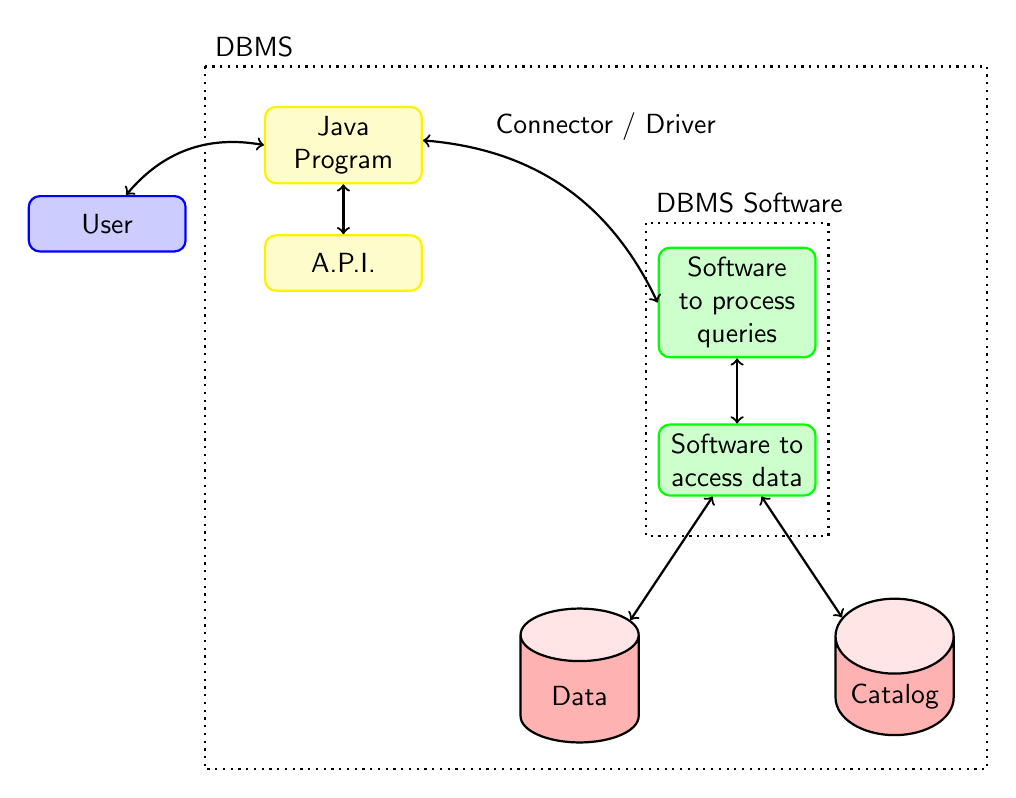
\begin{tikzpicture}[ 
    block/.style={
      rectangle,
      thick,
      text width=5em,
      align=center,
      rounded corners,
      minimum height=2em
    },
	data/.style={
		cylinder,
		draw=black,
		thick,
		aspect=0.7,
		minimum height=1.7cm,
		minimum width=1.5cm,
		shape border rotate=90,
		cylinder uses custom fill,
		cylinder body fill=red!30,
		cylinder end fill=red!10
	}
]

\node [block, fill=blue!20, draw=blue] (user) at (0,0) {User};
\node [block, fill=yellow!20, draw=yellow] (program) at (3,1) {Java Program};
\node [block, fill=yellow!20, draw=yellow] (api) at ($(program.south)+(0, -1)$) {A.P.I.};
\node [block, fill=green!20, draw=green] (process) at (8, -1) {Software to process queries};
\node [block, fill=green!20, draw=green] (access) at (8, -3) {Software to access data};
\node [data] (data) at (6, -6) {Data};
\node [data] (metadata) at (10, -6) {Catalog};

%% Frame

\draw[thick,dotted] ($(program.north west)+(-0.75,0.5)$) node[above right]{DBMS} rectangle ($(metadata.south east)+(0.75,-0.5)$) ;
\draw[thick,dotted] ($(process.north west)+(-0.15,0.3)$) node[above right]{DBMS Software} rectangle ($(access.south east)+(0.15,-0.5)$) ;
%% Arrows

\draw [<->, thick] (user) to [bend left] (program.west);
\draw [<->, thick] (program.south) to (api.north);
\draw [<->, thick] (program) to [bend left] node[above right, pos=0.2]{Connector / Driver} (process.west);
\draw [<->, thick] (process) to (access);
\draw [<->, thick] (access) to (data);
\draw [<->, thick] (access) to (metadata);

	\end{tikzpicture}
	

\end{document}